\scanpage{21}

% L1–3 upper left
\diagram{\begin{tikzcd}[ampersand replacement=\&,column sep=small,row sep=3ex]
 \& \underline{\unsure{\zeta|\xi}_1}\zeta_2\zeta_3
 \arrow[r,dash]\arrow[dl,dash]\arrow[dd,dash,dashed]\arrow[drr,dash,dashed]
 \& \underline{\zeta_4}\zeta_5\zeta_6
 \arrow[dr,dash]\arrow[dll,dash,dashed]\arrow[dd,dash,dashed] \& {}\\
 \underline{\zeta_{45}}\zeta_{56}\zeta_{64}\arrow[dr,dash]\arrow[drr,dash,dashed]
 \& \& \& \zeta_{23}\underline{\zeta_{31}}\zeta_{12}\arrow[dl,dash]\arrow[dll,dash,dashed]\\
 \& \underline{\zeta_{\deleted{\unsure{4}}1}^{\unsure{*|+}}}\zeta_2^*\zeta_3^*
 \arrow[r,dash]\& \underline{\zeta_4}\zeta_5^*\zeta_6^* \&
\end{tikzcd}}

% L1 top centre
\figure{\begin{tikzpicture}[scale=.5]\draw[->] (0,.6) .. controls (.45,.7) and (.8,.45) .. (1.1,0);\end{tikzpicture}}

% L1–2 upper right
\figure{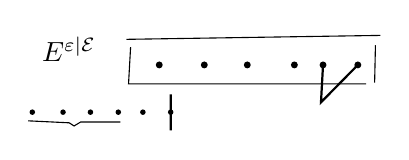
\begin{tikzpicture}[x=.52cm,y=.5cm]
\node at (-1,1.6) {$E^{\unsure{\varepsilon|\mathcal E}}$};
\draw (.4,1.85)--(6.6,1.95) (.5,1.65)--(.45,.72)--(6.25,.72) (6.48,1.7)--(6.46,.75);
\foreach \x in {1.2,2.3,3.35,4.5,5.2,6.05}{\fill (\x,1.2) circle (1.25pt);}
\foreach \x in {-1.9,-1.15,-.48,.2,.8,1.48}{\fill (\x,0) circle (1pt);}
\draw[thick] (5.2,1.2)--(5.15,.25)--(6.05,1.2) (1.48,.45)--(1.48,-.46);
\draw (-2,-.22)--(-1,-.27)--(-.88,-.35)--(-.72,-.25)--(.25,-.25);
\end{tikzpicture}}

% L3–4 upper right
(hexagone distingué ou triplet distingué

% L4 just below hexagon
$\unsure{\zeta_{14}|\zeta_1\,4}$

% L5–7 left
\deleted{2 ens à trois él. $E,E'$}

1 ens à trois él. $I$

% L7 left
\[
 E\times I\ \amalg\ E\times I'
\]

% L5–7 right
\[
\left\{\begin{aligned}
 &\text{ens à }\deleted{\unsure{3}}\!6\ \text{él. fibré \inserted{de degré 3} sur ens }\varepsilon\text{ à 2 él.}\\
 &\hspace{2em} E=\deleted{\unsure{E}}\coprod_{\alpha\in\varepsilon}E_\alpha\\
 &\text{ens à trois él. }I
\end{aligned}\right.
\]

% L8
\[
 I\times\varepsilon\quad\text{h\deleted{\unsure{a}}exagone}
\]

% L9 left
$\zeta_1\zeta_2\zeta_3$

% L9–12 centre
il y a 6 él. liés à aucun \uline{des $\zeta_i$}

il y a \unsure{3 él.|trois él.} \deleted{\unsure{sont}} liés à deux \unsure{$\zeta_\alpha$} \unsure{(pt E|$\alpha\in E$}

il y a 6 él. liés à exact 2 des $\zeta_i$

et 9 él. liés à exact un

% L9 right
\[
 E_\alpha\times I= E\mathbin{\unsure{\times|\alpha}}I\quad\text{fibré sur } I\mathbin{\times}\varepsilon
\]

% L12 lower centre
\[
 X=\prod_{\alpha\in\varepsilon}E_\alpha
\]

% foot, left to right
\figure{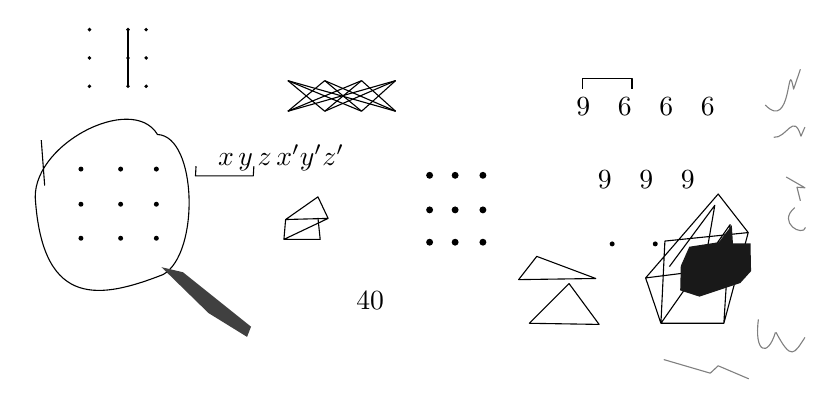
\begin{tikzpicture}[x=.72cm,y=.72cm,line join=round]
\foreach \x in {1.1,1.78,2.1}{\foreach \y in {4.4,4.9,5.4}{\fill (\x,\y) circle (.7pt);}}
\draw (1.78,4.4)--(1.78,5.4);
\draw (.15,2.35) .. controls (.02,3.35) and (1.85,4.3) .. (2.3,3.55) .. controls (3,3.52) and (3.05,1.45) .. (2.4,1.08) .. controls (1.3,.65) and (.3,.48) .. (.15,2.35);
\draw (.25,3.45)--(.31,2.65);
\foreach \x in {.95,1.65,2.28}{\foreach \y in {1.72,2.32,2.94}{\fill (\x,\y) circle (.9pt);}}
\fill[black!75] (2.37,1.21)--(2.75,1.12)--(3.95,.16)--(3.88,-.02)--(3.2,.4)--cycle;

\node at (4.48,3.14) {$x\,y\,z\,x'y'z'$};
\draw (2.98,2.99)--(2.97,2.82)--(3.99,2.82)--(4,2.99);
\foreach \x/\t in {4.6/5.25,4.6/5.9,4.6/6.5,5.25/4.6,5.25/5.9,5.25/6.5,5.9/4.6,5.9/5.25,5.9/6.5,6.5/4.6,6.5/5.25,6.5/5.9}{\draw[thin] (\x,4.5)--(\t,3.96);}
\draw (4.53,1.7)--(4.56,2.05)--(5.13,2.45)--(5.31,2.07)--(4.56,2.05) (5.31,2.07)--(4.53,1.7)--(5.17,1.7)--(5.13,2.08);
\foreach \x in {7.1,7.55,8.04}{\foreach \y in {1.65,2.22,2.83}{\fill (\x,\y) circle (1.25pt);}}
\node at (6.05,.62) {$40$};
\node at (10.91,4.04) {$9\quad 6\quad 6\quad 6$};
\draw (9.8,4.36)--(9.8,4.54)--(10.67,4.54)--(10.67,4.36);
\node at (10.92,2.76) {$9\quad 9\quad 9$};
\fill (10.32,1.62) circle (.9pt); \fill (11.08,1.62) circle (.9pt);
\draw (8.67,.99)--(8.99,1.4)--(10.03,1.01)--cycle (8.86,.22)--(9.56,.92)--(10.09,.2)--cycle;
\draw (10.91,1.02)--(12.19,2.5)--(12.72,1.82)--(12.29,.22)--(11.18,.22)--cycle
 (11.18,.22)--(11.25,1.67)--(12.72,1.82) (10.91,1.02)--(12.5,1.22)
 (11.18,.22)--(12.4,1.96)--(12.29,.22) (11.33,1.22)--(12.13,2.3)--(11.92,1.08);
\fill[black!90] (11.53,1.23)--(11.68,1.57)--(12.2,1.65)--(12.43,1.95)--(12.45,1.63)--(12.76,1.63)--(12.77,1.14)--(12.58,.93)--(11.86,.69)--(11.52,.8)--cycle;
\draw[gray,thin] (13.02,4.07) .. controls (13.5,3.58) and (13.4,4.98)..(13.52,4.35)--(13.64,4.7)
 (13.17,3.5) .. controls (13.4,3.48) and (13.52,3.95)..(13.65,3.52)--(13.72,3.68)
 (13.39,2.8)--(13.72,2.61)--(13.58,2.62)--(13.64,2.38)
 (13.54,2.26) .. controls (13.22,1.99) and (13.69,1.74)..(13.73,1.91)
 (12.9,.29) .. controls (12.82,-.29) and (13.06,-.4)..(13.2,.06)
 (13.21,.06) .. controls (13.48,-.45) and (13.53,-.32)..(13.72,-.03)
 (11.23,-.42)--(12.05,-.66)--(12.19,-.53)--(12.73,-.76);
\end{tikzpicture}}
% crop-candidate: scan 21
% archive sheet number: 20
